\documentclass{article}
\usepackage{amsmath}
\usepackage{amssymb}
\usepackage{booktabs}
\usepackage{xintexpr}
\usepackage{tikz}
\usetikzlibrary{arrows,automata}

\newcommand{\T}{1}
\newcommand{\F}{0}
\newcommand{\TF}[1]{\if1#1\T\else\F\fi}
\newcommand{\xintTF}[1]{\xintifboolexpr{#1}{\T}{\F}}

\newcommand{\logicrule}[2]{
\begin{array}{l}
#1 \\
\midrule
\therefore #2 \\
\end{array}
}

\newcommand{\inv}[1]{#1^{-1}}

\renewcommand{\d}[1]{\,\textnormal{d}#1}
\newcommand{\dd}[2]{\frac{\d{#1}}{\d{#2}}}
\newcommand{\ddd}[2]{\dfrac{\d{#1}}{\d{#2}}}

\DeclareMathOperator{\var}{Var}
\DeclareMathOperator{\E}{\mathcal{E}}

\newcommand{\multistep}[1]{\begin{array}{rl} #1 \end{array}}
\newcommand{\subeq}{\subseteq}
\newcommand{\sub}{\subset}

\newcommand{\conj}[1]{\overline{#1}}

\setlength\parindent{0pt}
\setlength\parskip{1em}

\begin{document}

\section*{Quiz}

A property whose domain is a set of k-tuples
$A\times{}A\times\cdots\times{}A$ is a \textbf{relation}.

The binary operation that is symmetric is: $x=y$.

A binary relation that is reflexive, smmetric, and transitive is
called an \textbf{equivalence relation}.

\section*{Strings}

A string over an alphabet is a finite sequence of symbol.

If $w$ is a string over $\Sigma$, the length of $w$ (written as $|w|$)
is the number of symbols.

Strings of length zero are ``empty strings'' (written as $\epsilon$).

If $|w|=n$, then $w$ can be written as $a_1a_2\cdots{}a_n$ where each
$a_i\in\Sigma$ for $i=1,2,\cdots,n$.

\subsection*{String Operations}

The \textbf{reverse} of $w$ (written as $w^R$), where
$w=w_1w_2\cdots{}w_n$, is $w^R=w_nw_{n-1}\cdots{}w_2w_1$.

The string $z$ is a \textbf{substring} of $w$ if $w=xzy$ for $x$, $y$
not necessarily empty strings. $x$ and $y$ are \textbf{prefixes} and
\textbf{suffixes}, respectively.

\textbf{Concatenation} of two strings $x=x_1x_2\cdots{}x_m$ and
$y=y_1y_2\cdots{}y_n$ is defined as
$xy=x_1x_2\cdots{}x_my_1y_2\cdots{}y_n$.

A string $x$ can be \textbf{repeated} $k$ times is defined as
$x^k=\underbrace{xx\cdots{}x}_{\text{$x$ times}}$.

\textbf{Lexicographic ordering} is more commonly known as ``dictionary
ordering''.

\section*{Formal Language}

A formal language is a set of strings over a given alphabet.

\subsection*{Problems/Issues}

\begin{enumerate}
\item How do you specify a language?
\item How do you recognize the strings?
\item How do you translate the language?
\end{enumerate}

\subsection*{Regular Languages}

Using our problem abstraction:

\begin{description}
\item[Data] a word in a given language. $\Sigma$ and $\Sigma^*$.
\item[Conditions] set of words is a language. $L\subseteq\Sigma^*$ is
  a formal language.
\item[Unknown] boolean variable. true if word is in a language, false
  otherwise. Given that $w\in\Sigma^*$ and $L\subseteq\Sigma^*$, is
  $w\in{}L$?
\end{description}

\section*{Finite Automata (FA)}

Also called a ``finite state machine'' (FSM). We can represent all of
this using either: graphics, tables, or mathematics.

\subsection*{Formal Definition}

Every FA can be represented as a $5$-tuple $(Q,\Sigma,\delta,q_0,F)$,
where:

\begin{description}
\item[$Q$]: finite set (states)
\item[$\Sigma$]: finite set (alphabet)
\item[$\delta$]: $Q\times\Sigma\rightarrow{}Q$ (transition function)
\item[$q_0\in{}Q$]: start state (initial state)
\item[$F\subseteq{}Q$]: set of accept states (final states)
\end{description}

\subsection*{Applications}

\begin{itemize}
\item Compilers
\item Pattern recognition
\item Speech Processing/OCR
\item Modeling/predicting price/stock changes in finance
\end{itemize}

\subsection*{Computation: Abstract}

\begin{enumerate}
\item Receives input symbols. One by one. Left to right.
\item After reading each symbol, our machine $M_1$ moves from one
  state to another according to transition function.
\item After $M_1$ reads last symbol of input, it produces the
  output. We accept the output if $M_1$ is in an accept state,
  otherwise we reject.
\end{enumerate}

\subsection*{Language Recognized by FA}

If $P$ is the set of strings that FA $M$ accepts, then $P$ is the
language of the machine $M$ , which we write as $L(M)=P$.

The FA may accept several strings, but always recognizes only one
language.

If the machine accepts no strings, then it recognizes the empty
language $\varnothing$.

\subsection*{Computation: Mathematics}

Let $M=(Q,\Sigma,\delta,q_0,F)$ be a FA.

Let $w=a_1a_2\cdots{}a_n$ be a string over $\Sigma$.

$M$ accepts $w$ if there is a sequence of states $r_0r_1\cdots{}r_n$
exist in $Q$ such that the following holds:

\begin{enumerate}
\item $r_0=q_0$
\item $r_{i+1}=\delta(r_i, q_{i+1})$ for $i=0,1,\cdots,n-1$
\item $r_n\in{}F$
\end{enumerate}

\subsection*{Regular Language}

FA $M$ recognizes the language $L$ if $L=\{w|\text{$M$ accepts $w$}\}$.

A language is called ``regular'' if there exists an FA that recognizes
it.

\subsection*{Example}

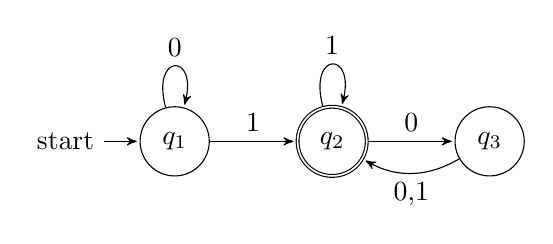
\begin{tikzpicture}[>=stealth',shorten >=1pt,auto,node distance=2cm]
  \node[initial,state] (q1)      {$q_1$};
  \node[state,accepting]         (q2) [right of=q1]  {$q_2$};
  \node[state]         (q3) [right of=q2] {$q_3$};

  \path[->] (q1) edge [loop above] node {0} (q1)
  (q1) edge node {1} (q2)
  (q2) edge [loop above] node {1} (q2)
  (q2) edge node {0} (q3)
  (q3) edge [bend left] node {0,1} (q2);
\end{tikzpicture}

$M: (Q,\Sigma,\delta,q_1,F)$

\begin{description}
\item[$Q$] $= \{q,1,q_2,q_3\}$
\item[$\Sigma$] $= \{0,1\}$
\item[$\delta$] rawr
\end{description}


\end{document}
